% !TeX root = ../main.tex
\clearpage
\subsection{تمرین \secnum{۴.۱۰}، دو پیاده‌سازی گیت \lr{AND}}
\label{sec:delay-exercise-and2}

\textbf{خواسته.}
دو مدار شکل \secnum{۴.۳۹} کتاب را مقایسه کنید. برای هر مدار
\lr{Path Effort} و کمینه تأخیر را حساب کنید و ظرفیت‌های
ورودی \(x\) و \(y\) را به دست آورید
\cite[تمرین \secnum{۴.۱۰} و شکل \secnum{۴.۳۹}، صفحه ۱۷۷]{weste}.

\textbf{خواندن مدار.}
در شکل \ref{fig:delay-exercise-and2-paths}، طرح \lr{(a)}
با یک \lr{NAND2} و یک \lr{Inverter} ساخته شده است.
در طرح \lr{(b)}، دو ورودی جداگانه وارونه می‌شوند و به
دو پایه گیت پایانی می‌روند. گیت پایانی در شکل کتاب، نماد
\lr{AND} با حباب در هر دو ورودی دارد. اگر \(U\) و \(V\)
سیگنال‌های رسیده به آن باشند، خروجی
\(\overline U\cdot\overline V=\overline{U+V}\) است.
بنابراین این گیت از دید اندازه‌گذاری به‌صورت \lr{NOR2}
مدل می‌شود. از هر ورودی تا خروجی فقط یکی از
\lr{Inverter}های طرح \lr{(b)} در مسیر قرار می‌گیرد.

\begin{figure}[htbp]
  \centering
  \begin{latin}
  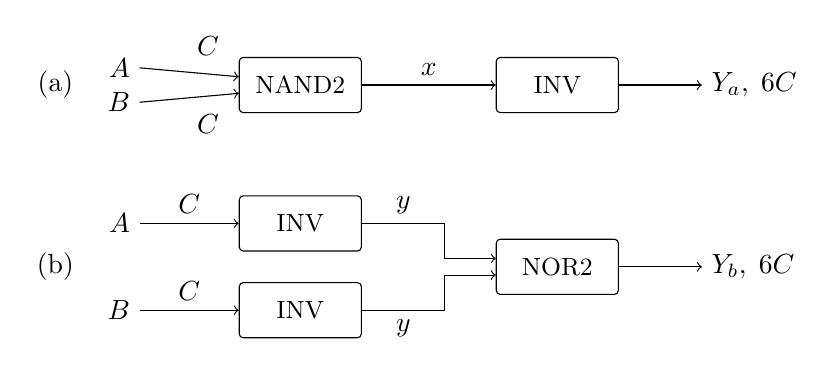
\begin{tikzpicture}[x=1.02cm,y=0.95cm,
      gate/.style={draw,rounded corners=1.4pt,minimum width=1.55cm,
        minimum height=0.7cm,align=center,font=\small}]
    \node at (0.05,1.85) {(a)};
    \node[gate] (nand) at (3.1,1.85) {NAND2};
    \node[gate] (tail) at (6.3,1.85) {INV};
    \draw[->] (1.1,2.08) node[left] {\(A\)}
      -- ([yshift=3pt]nand.west);
    \draw[->] (1.1,1.62) node[left] {\(B\)}
      -- ([yshift=-3pt]nand.west);
    \draw[->] (nand.east) -- (tail.west) node[midway,above] {\(x\)};
    \draw[->] (tail.east) -- (8.1,1.85) node[right] {\(Y_a,\;6C\)};
    \node[above] at (1.95,2.11) {\(C\)};
    \node[below] at (1.95,1.59) {\(C\)};
    \node at (0.05,-0.58) {(b)};
    \node[gate] (invA) at (3.1,0) {INV};
    \node[gate] (invB) at (3.1,-1.16) {INV};
    \node[gate] (nor) at (6.3,-0.58) {NOR2};
    \draw[->] (1.1,0) node[left] {\(A\)} -- (invA.west)
      node[midway,above] {\(C\)};
    \draw[->] (1.1,-1.16) node[left] {\(B\)} -- (invB.west)
      node[midway,above] {\(C\)};
    \draw[->] (invA.east) -- (4.9,0) node[midway,above] {\(y\)}
      |- ([yshift=3pt]nor.west);
    \draw[->] (invB.east) -- (4.9,-1.16) node[midway,below] {\(y\)}
      |- ([yshift=-3pt]nor.west);
    \draw[->] (nor.east) -- (8.1,-0.58) node[right] {\(Y_b,\;6C\)};
  \end{tikzpicture}
  \end{latin}
  \caption{دو پیاده‌سازی \lr{AND} دوورودی، بازترسیم‌شده از
  شکل \secnum{۴.۳۹} کتاب \cite{weste}. \(C\) ظرفیت هر
  ورودی خارجی، \(6C\) بار خروجی، \(x\) ظرفیت ورودی
  \lr{Inverter} پایانی و \(y\) ظرفیت هر ورودی \lr{NOR2}
  است.}
  \label{fig:delay-exercise-and2-paths}
\end{figure}

\textbf{محاسبه تأخیر و اندازه‌ها.}
در \(F=GBH\)، \(F\) همان \lr{Path Effort} و \(G\)
حاصل‌ضرب \lr{Logical Effort} گیت‌های مسیر است. \(B\)
حاصل‌ضرب نسبت بار کل به بار روی مسیر در هر مرحله و
\(H\) نسبت بار انتهایی به ظرفیت ورودی مسیر است.
هر مسیر در هر دو طرح دو مرحله دارد. ظرفیت ورودی همان مسیر
\(C\)، بار خروجی \(6C\) و \(H=6\) است. هر خروجی میانی
فقط یک پایه از گیت بعدی را راه‌اندازی می‌کند، پس \(B=1\).
با \(p=1\) برای \lr{Inverter} و \(p=2\) برای گیت دوورودی، مجموع تأخیر
\lr{Parasitic} در هر دو طرح \(P=3\) است. تفاوت اصلی در
\(G\) است.
با ضرب \(g_i\)های مسیر برای \(G\) و جای‌گذاری در \(F=GBH\) داریم.\[
  G_a=\frac43\cdot1,\quad F_a=8,
  \qquad
  G_b=1\cdot\frac53,\quad F_b=10.
\]
در طرح \lr{(a)}، ترانزیستورهای سریِ گیت دوورودی از نوع
\lr{nMOS} هستند. گیت دوورودی طرح \lr{(b)} برای دستیابی
به قدرت راه‌اندازی مشابه، به \lr{pMOS}های سری عریض‌تر
نیاز دارد. ظرفیت ورودی بیشترِ گیت هم‌قدرت در \(G_b\) بزرگ‌تر
ظاهر می‌شود.
با برابرگرفتن سهم وابسته به بار هر مرحله با \(\sqrt F\)، تأخیرهای
بهینه چنین‌اند.
\[
  D_{\min,a}=2\sqrt{8}+3\approx8.66,
  \qquad
  D_{\min,b}=2\sqrt{10}+3\approx9.32.
\]
ظرفیت هر گیت پایانی با تنظیم سهم وابسته به بارِ آن روی
\(\widehat f=\sqrt F\) به دست می‌آید.
با حل \(g_i C_L/C_{\mathrm{in}}=\widehat f\) برای ظرفیت
ورودی گیت پایانی داریم.\[
  x=\frac{6C}{\sqrt8}\approx2.12C,
  \qquad
  y=\frac{(5/3)6C}{\sqrt{10}}=\sqrt{10}\,C\approx3.16C.
\]
برای کنترل اندازه‌ها، سهم مرحله اول در طرح \lr{(a)}
برابر \((4/3)(x/C)=\sqrt8\) و در طرح \lr{(b)} برابر
\(y/C=\sqrt{10}\) است. بنابراین در هر طرح دو مرحله
\lr{Stage Effort} برابر دارند و برای بار و ظرفیت ورودی
داده‌شده، طرح \lr{(a)} سریع‌تر است.
